\documentclass[oneside,a4paper]{memoir}

\usepackage[T1]{fontenc}
\usepackage{microtype}
\usepackage{graphicx}
\usepackage{subcaption}
\usepackage{textcomp}
\usepackage{enumitem}

\usepackage{libertine}
\usepackage{libertinust1math}
\usepackage{inconsolata}

\usepackage{menukeys}

\usepackage{minted}
\setminted{frame=lines}
% from https://tex.stackexchange.com/a/368971/155372
\newenvironment{longlisting}{\captionsetup{type=listing}}{}

\usepackage{hyperref}
\usepackage{xcolor}
\hypersetup{
    colorlinks,
    linkcolor={red!80!black},
    citecolor={red!50!black},
    urlcolor={blue!50!black},
    filecolor={blue!50!black}
}

\usepackage{tikz}
\usetikzlibrary{arrows.meta}

\chapterstyle{bianchi}
% Changing the fonts a bit
\renewcommand*{\chapnamefont}{\normalfont\huge\itshape}
\renewcommand*{\chaptitlefont}{\normalfont\Huge}

% Adapted from https://tex.stackexchange.com/a/315324/155372
\newcommand{\grid}[2][blue!75]{
\fill[#1]
  \foreach \row [count=\y] in {#2} {
    \foreach \cell [count=\x] in \row {
      \ifnum\cell=1 %
        (\x-1, -\y+1) rectangle ++(1, -1)
      \fi
      \pgfextra{%
        \global\let\maxx\x
        \global\let\maxy\y
      }%
    }
  }
;
\draw[thin] (0, 0) grid[step=1] (\maxx, -\maxy);
}

\newcommand\hreftt[2]{\href{#1}{\texttt{#2}}}

\begin{document}

\title{Cabasa: User Manual}
\preauthor{}\postauthor{}\author{} % removes extra space when no author is given
\maketitle

\tableofcontents

\chapter{Introduction}

Cabasa is an application for the simulation of arbitrary 2D cellular automata.

\section{What is a Cellular Automaton?}
\label{sec:whatisca}

\textbf{Note:} You can skip this section if you already know about cellular automata.

\vspace{2ex}

A \emph{cellular automaton} (abbreviated from now on as CA/CAs) is a type of mathematical simulation which operates on a set of \emph{cells}.
The cells are arranged in some sort of lattice (typically a 1D line or a 2D grid).
Each cell has an associated \emph{state}, which is one value drawn from a predefined set of values.

On each step of the simulation, a fixed set of rules is applied.
Each step is referred to as a \emph{generation}.
A pattern starts at generation 0, and each time the rules are applied the generation is increased by one.

To illustrate this, consider the well-known CA known as \emph{Conway's Game of Life} (or \emph{Life} for short).
This CA takes place on a 2D grid.
Each cell in this grid has a state drawn from a set of two states, usually called `Alive' and `Dead'.
Each generation, the grid evolves according to the following rules:

\begin{enumerate}
\item \label{itm:gold3} If the current cell is dead but exactly three of the surrounding cells are alive, then the cell becomes alive.
\item \label{itm:goldo} Otherwise a dead cell stays dead.
\item \label{itm:gola23} If the current cell is alive and two or three of the surrounding cells are alive, then the cell stays alive.
\item \label{itm:golao} Otherwise a live cell turns into a dead cell.
\end{enumerate}

\begin{figure}
  \centering
  \begin{subfigure}{\linewidth}
    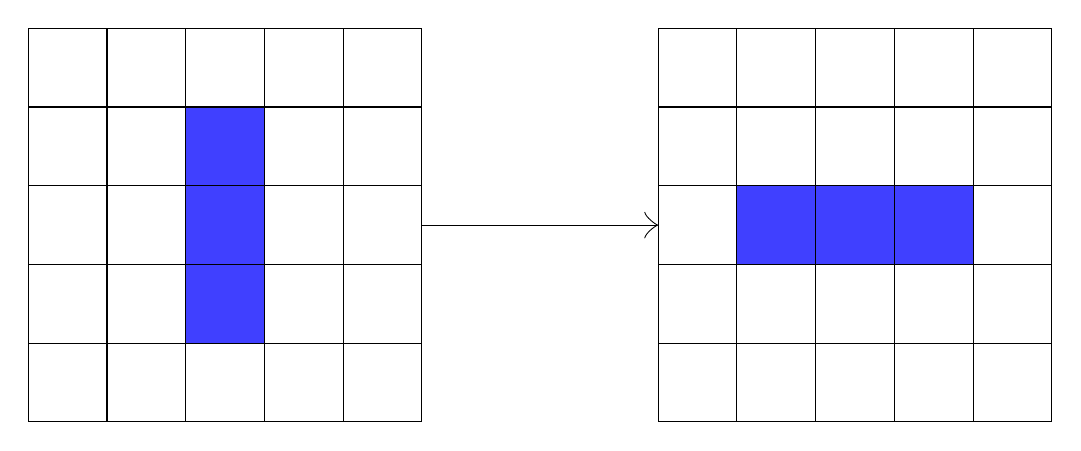
\begin{tikzpicture}
      \begin{scope}[xshift=-4cm]
        \grid{
          {0,0,0,0,0},
          {0,0,1,0,0},
          {0,0,1,0,0},
          {0,0,1,0,0},
          {0,0,0,0,0}}
        \node(arrstart) at (5,-2.5) {};
      \end{scope}
      \begin{scope}[xshift=4cm]
        \grid{
          {0,0,0,0,0},
          {0,0,0,0,0},
          {0,1,1,1,0},
          {0,0,0,0,0},
          {0,0,0,0,0}}
        \node(arrend) at (0,-2.5) {};
      \end{scope}
      \draw[-{Classical TikZ Rightarrow[length=5pt]}] (arrstart.center) -- (arrend.center);
    \end{tikzpicture}
    \subcaption{The pattern itself}
  \end{subfigure}\\
  \begin{subfigure}{\linewidth}
    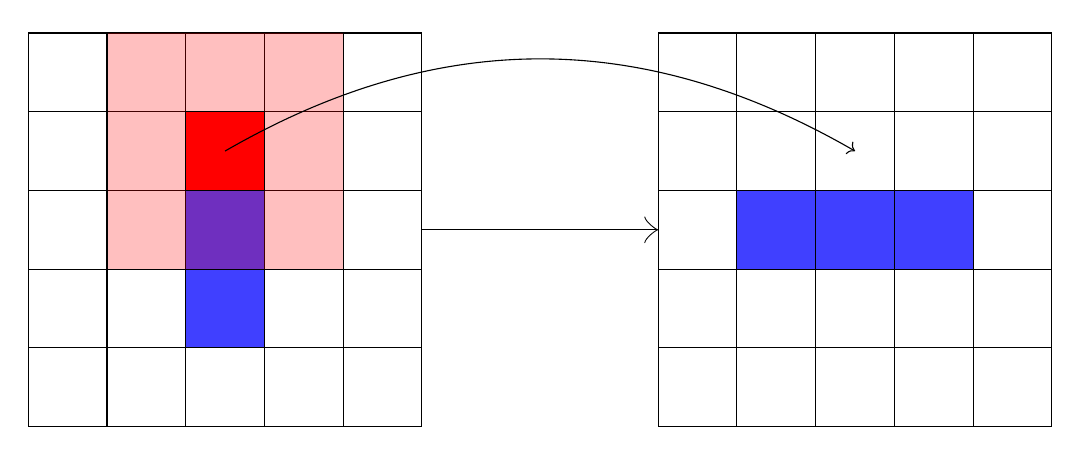
\begin{tikzpicture}
      \begin{scope}[xshift=-4cm]
        \grid{
          {0,0,0,0,0},
          {0,0,1,0,0},
          {0,0,1,0,0},
          {0,0,1,0,0},
          {0,0,0,0,0}}
        \node(arrstart) at (5,-2.5) {};
        \node(first) at (2.5,-1.5) {};
        \draw[fill=red,fill opacity=0.25] (1,0) rectangle ++(3,-3);
        \draw[fill=red] (2,-1) rectangle ++(1,-1);
      \end{scope}
      \begin{scope}[xshift=4cm]
        \grid{
          {0,0,0,0,0},
          {0,0,0,0,0},
          {0,1,1,1,0},
          {0,0,0,0,0},
          {0,0,0,0,0}}
        \node(arrend) at (0,-2.5) {};
        \node(second) at (2.5,-1.5) {};
      \end{scope}
      \draw[-{Classical TikZ Rightarrow[length=5pt]}] (arrstart.center) -- (arrend.center);
      \draw[->] (first.center) to[bend left] (second.center);
    \end{tikzpicture}
    \subcaption{With a live cell highlighted}
    \label{fig:GoLli}
  \end{subfigure}
  \begin{subfigure}{\linewidth}
    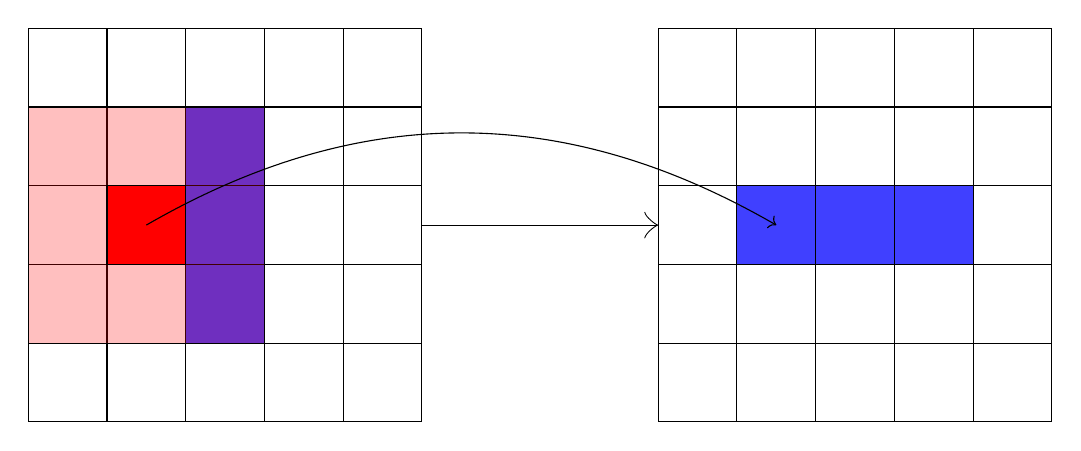
\begin{tikzpicture}
      \begin{scope}[xshift=-4cm]
        \grid{
          {0,0,0,0,0},
          {0,0,1,0,0},
          {0,0,1,0,0},
          {0,0,1,0,0},
          {0,0,0,0,0}}
        \node(arrstart) at (5,-2.5) {};
        \node(first) at (1.5,-2.5) {};
        \draw[fill=red,fill opacity=0.25] (0,-1) rectangle ++(3,-3);
        \draw[fill=red] (1,-2) rectangle ++(1,-1);
      \end{scope}
      \begin{scope}[xshift=4cm]
        \grid{
          {0,0,0,0,0},
          {0,0,0,0,0},
          {0,1,1,1,0},
          {0,0,0,0,0},
          {0,0,0,0,0}}
        \node(arrend) at (0,-2.5) {};
        \node(second) at (1.5,-2.5) {};
      \end{scope}
      \draw[-{Classical TikZ Rightarrow[length=5pt]}] (arrstart.center) -- (arrend.center);
      \draw[->] (first.center) to[bend left] (second.center);
    \end{tikzpicture}
    \subcaption{With a dead cell highlighted}
    \label{fig:GoLdi}
  \end{subfigure}
  \caption{Evolving a pattern by one generation using Conway's Game of Life}
  \label{fig:GoL}
\end{figure}

The effect of these rules can be seen in Figure~\ref{fig:GoL},
  which shows the effect of one application of the above rules on a small starting pattern.
Dead cells are drawn in white and live cells are drawn in blue.

To illustrate the rules more clearly, in Figure~\ref{fig:GoLli} one live cell is highlighted in red.
Its eight surrounding cells are highlighted in a lighter colour.
If we consider the middle cell, we can see that it is next to only one live cell,
  so by the Rule~\ref{itm:golao} above it turns into a dead cell.
Figure~\ref{fig:GoLdi} is similar, except that a dead cell is highlighted instead of a live cell.
This cell has three neighbouring live cells, so by Rule~\ref{itm:gold3} it becomes alive in the next generation.

\section{About Cabasa}
\label{sec:about}

Cabasa is an application for running \textbf{2D} cellular automata on (at the moment) a \textbf{finite} grid.
It aims to support any CA, unlike existing applications which can only support certain classes of CAs.
Do note that it does not aim to be particularly fast; if you want a very fast simulator, another application is probably better.

\chapter{Quickstart}
\label{chap:qstart}

To select a new rule, press the \menu{Control > Set Rule} menu item.
This opens a rule-selection dialog, where you can type a rule in or select a preexisting rule.
Cabasa comes with a set of predefined rules; to select one of these, use the menu item \menu{File > Open}.
In this example, we'll use the \texttt{life.alp} rule; it implements the \emph{Game of Life} rule described in Section~\ref{sec:whatisca}.
Selecting this rule and pressing the `Ok' button will make its contents appear in the dialog.
Press the \texttt{Set Rule} button to change the current rule to the rule which you have selected.

Now we can draw a pattern on the grid to use with this rule.
Select state \texttt{1} from the dropdown box at the top of the window marked `Current drawing state' (see screenshot, Figure~\ref{fig:mainwin}).
After this you should be able to draw patterns on the grid.
If you press the \keys{M} key, you can click and drag to move around; pressing \keys{D} gets you back to drawing mode.

To run the selected CA rule on your pattern, press the triangular `Play' button on the left of the screen;
  pressing it again should pause the evolution.
You should observe the pattern changing;
  this is due to the repeated application of the \emph{Game of Life} rules as described above.

\chapter{Getting Started}
\label{chap:gstart}

\section{User interface}
\label{sec:ui}

\begin{figure}[h]
  \centering
  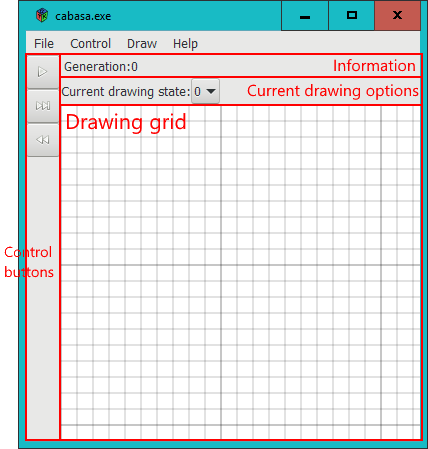
\includegraphics[scale=.8]{screenshot.png}
  \caption{Cabasa Main Window}
  \label{fig:mainwin}
\end{figure}

The main window, shown on Figure~\ref{fig:mainwin}, is composed of several parts.

The large grid in the middle shows the current state of the CA grid.
The user can draw on the grid, move around to show the rest of the grid, and use the currently loaded CA to evolve the pattern shown on the grid.

The information pane, just below the menu, shows various pieces of information about the current application state.
Currently it only shows the current generation,
  but it is expected that it will contain more information in future versions of Cabasa.

The drawing options pane, below the information pane, shows options related to drawing.
Again, there is currently only one thing shown here, but future versions may add more.
This pane will be disabled if drawing mode is not enabled.

\section{Drawing and Moving}
\label{sec:drming}

The application starts in \emph{drawing mode}.
In this mode, clicking and dragging on the grid changes the state of each cell the cursor passes over.

By default, the grid starts with all grid cells set to state 0 and the \emph{drawing state} also set to 0,
  so nothing happens when you try to draw on the grid.
However, by changing the selected state (next to the text `Current drawing state'), other states can be chosen.
For instance, if state 1 is selected, then clicking and dragging on the grid will change the cells under the cursor to state 1.
Note that the states are numbered starting from 0, not 1,
  so to select e.g.\ the second state you have declared you need to select state 1, not state 2.

Moving around the grid requires another mode, \emph{move mode}.
This mode can be selected from the \menu{Draw > Mode} menu, or by pressing the \keys{M} key.
You can get back to drawing mode by using the \menu{Draw} menu, or by pressing the \keys{D} key.
In this mode, clicking and dragging will not draw on the grid, but rather will move or pan around the grid.
Enabling this mode will also disable the `drawing options' pane.

In any mode, you can also zoom in and out using the mouse wheel.
Scroll up over a point to zoom in to that point, and scroll down to zoom out.

If you zoom out far enough, you will notice that the grid abruptly comes to an end at a certain point.
This is because the grid is finite.
However, the grid `wraps around' at its edges; that is, if you move off one edge of the grid, you reappear at the opposite edge.
For instance, the cell immediately above the topmost cell is considered to be the bottommost cell.

\section{Selection and copying}
\label{sec:selcopy}

In addition to the two modes described above, there is also a mode for selecting parts of the grid.
This \emph{selection mode} may be accessed via the \menu{Draw > Mode} menu, like the other two modes,
  or with the \keys{S} hotkey.
In this mode, you may click and drag to select a portion of the grid (shown in green).
Click and drag again in a different part of the grid to make a new selection.
To clear the current selection, use the \hbox{\menu{Draw > Clear Selection}} menu item,
  or its hotkey \keys{\ctrl + K}.

Once you have selected part of a grid, you may \emph{copy} it into the \emph{clipboard},
  with the purpose of \emph{pasting} it back into another part of the grid.
To copy the selection, use the \menu{Edit > Copy} menu item.
To paste your selection back, press \menu{Edit > Paste};
  a brown overlay will then be shown at the location where your selection will be pasted.
Move your mouse, and then click on your document to paste your selection at the shown location.
The usual hotkeys \keys{\ctrl + C} and \keys{\ctrl + V} respectively may also be used.

\section{Changing the Rule}
\label{sec:chngrule}

The current CA can be changed using the \menu{Control > Set Rule} menu item.
This opens a window where you can type in a specification of a CA rule.

Two specification languages are supported: \emph{ALPACA} and \emph{Haskell}.
You can switch between these using the option box at the bottom of the window.
For more details on these formats, see Chapter~\ref{chap:speccas}.

To accept a specification, press the `Set Rule' button at the bottom of the window.
This will interpret the specification and load it into the main window.
If the specification is invalid, it will show an error dialog instead.

After the rule is set, you will be able to draw patterns in this rule on the grid in the main window.
The set of states available for drawing through the `current drawing state' option will change to reflect the new rule.
Since the set of allowed states could have changed, the grid will be cleared after each rule change.

For more details on how to specify a CA, see Chapter~\ref{chap:speccas},
  but if you want to play around with a specification now then you can copy the following Game of Life specification into the `Set Rule' window:

\begin{verbatim}
state Dead  " "
  to Alive when 3 Alive and 5 Dead;
state Alive "*"
  to Dead when 4 Alive or 7 Dead.
\end{verbatim}

This is written in ALPACA, so make sure that the ALPACA language is selected before setting the rule.

\section{Running CAs}
\label{sec:running}

A set of \emph{control buttons} can be seen on the left of the window.
These buttons are used to actually run the CA once a rule has been loaded and a pattern has been drawn.

To run one generation of the CA, use the middle button.
This operation is called \emph{stepping}.
You can repeatedly press this button to run the rules more than once.

The topmost button will repeatedly step the CA when it is pressed once.
This operation is generally referred to as \emph{running} the CA.
After this button has been pressed, the icon will change to a pause icon.
As this suggests, the button can be pressed again to pause the CA.
Pressing it again will allow the CA to be run again.

To adjust the rate of running, use the \menu{Control > Faster} and \menu{Control > Slower} menu items.
Alternatively, you may press the \keys{{+}} or \keys{-} keys respectively.
The current speed is shown at the top of the window as the delay between steps;
  that is, a smaller number indicates a faster speed.
Do note that Cabasa will not let you increase the speed below 100,
  since at these fast speeds Cabasa may crash when it attempts to calculate too quickly.

To reset the CA after you have run or stepped it, use the bottom `reset' button.
This button will restore the original state of the CA after you have pressed the `step' or `run' buttons.
If you haven't run the CA, then it doesn't do anything.

To clear the pattern, use the \menu{Draw > Clear} menu item.
This resets the generation, clears the pattern and moves the grid so that the top-left corner is displayed
  (as in the start of the program).

\section{Opening and Saving}
\label{sec:opsav}

Cabasa has the ability to open and save both rules and patterns.
This can be done through the \menu{File > Open} and \menu{File > Save As} menu items on the CA specification window and main window respectively.
\textit{Save} (as opposed to \textit{save as}) functionality has not yet been implemented, but will be implemented in a later version of Cabasa.

In more detail:

\begin{itemize}
\item To \textbf{save the current rule}, use the \menu{Control > Set Rule} menu item on the main window to open the CA selection window.
  Then press the \menu{File > Save As} menu item on the CA selection window to show a file selection dialog where you can save the current rule.
  Ensure that the correct format (ALPACA or Haskell) is selected before saving.
\item To \textbf{open a previously saved rule}, use the \menu{Control > Set Rule} menu item on the main window to open the CA selection window.
  Then press the \menu{File > Open} menu item on the CA selection window to show a file selection dialog where you can open a previously saved rule.
  If your rule is not listed, try changing the file format (ALPACA or Haskell) at the bottom of the window.
  After the rule has been opened, press the \textit{Set Rule} button at the bottom of the window to load it as the current rule.
\item To \textbf{save the current pattern}, use the \menu{File > Save As} menu item on the main window to show a file selection dialog where you can save the current pattern.
\item To \textbf{open a previously saved pattern}, use the \menu{File > Open} menu item on the main window to show a file selection dialog where you can open a previously saved pattern.
  If the pattern has been saved with a different rule to the rule currently active,
    a dialog box will be shown asking you if you want to switch rules.
\end{itemize}

\subsection{Finding rules}
\label{sec:findrs}

If Cabasa needs to find a previously-saved rule (as may occur when e.g.\ opening a saved pattern),
  it uses the following steps to find it:

\begin{enumerate}
\item Inspect the folder specified by the \texttt{User-defined rules directory} setting (see Section~\ref{sec:sets});
  use the rule if it is found in this folder.
\item Inspect the folder specified by the \texttt{Predefined rules directory} setting (see Section~\ref{sec:sets});
  use the rule if it is found in this folder.
\item The rule could not be found in any known folder; ask the user if they want to find it manually.
\end{enumerate}

\section{Settings}
\label{sec:sets}

Cabasa can be customised through the use of various settings.
These can be accessed through the \menu{File > Settings} menu item.
The following settings are currently supported:

\begin{description}
\item[Predefined rules directory]
  The directory in which sample rules are stored.
  (See Section~\ref{sec:findrs} for details.)
\item[User-defined rules directory]
  The directory in which user-defined rules are stored.
  (See Section~\ref{sec:findrs} for details.)
\item[Default grid size]
  A default grid size of $x \times y$ causes the default grid to have a size of $x$ columns by $y$ rows.
  Note that changing this setting does \textit{not} have any effect on the current grid;
    it only takes effect if a new grid is made.
\end{description}

\chapter{Specifying CAs}
\label{chap:speccas}

\section{Languages}
\label{sec:speclangs}

Cabasa supports two languages to specify CAs: \emph{ALPACA} and \emph{Haskell}.

ALPACA is a language created by Chris Pressey specifically for the specification of CAs.
Cabasa currently supports ALPACA version 1.1.

Cabasa also allows CAs to be implemented in the Haskell programming language.
As Haskell is a full-featured programming language, this approach is more powerful than using ALPACA,
  but is extremely difficult if you do not already know Haskell.

\section{Using ALPACA}
\label{sec:usalp}

The reference manual for ALPACA version 1.1 is a very good guide for learning about the various features of ALPACA.
It is available at the following web address: \url{https://github.com/catseye/ALPACA/blob/0b2d57b8739dc240969c62c8e1cd13c1863770e0/doc/ALPACA.markdown}.
Cabasa should support all the features outlined in that manual
  \textbf{except} for the initial configuration, which is currently ignored.

Do note however that for technical reasons\footnotemark,
  the `examples' in the ALPACA manual are actually written in a format called `Falderal' and not plain ALPACA;
  the ALPACA translation can be found by reading the parts of the example which are after the \texttt{|} characters.
For instance, take this example from the manual:

\begin{verbatim}
| state Space " ";
| state Up "U"
|   to ^ when true;
| state Down "D"
|   to v when true
| begin
| DDD
| UUU
= -----
= UUU
= DDD
= -----
\end{verbatim}

For this example, the ALPACA which you would actually type is the following portion:

\begin{verbatim}
state Space " ";
state Up "U"
  to ^ when true;
state Down "D"
  to v when true
begin
DDD
UUU
\end{verbatim}

\footnotetext{In more detail: the `examples' are actually runnable tests containing an embedded description of the expected output as well.}

\section{Using ALPACA Stylesheets}
\label{sec:stys}

The \emph{ALPACA Stylesheets} format is a simple way to change the styling of a CA specified using ALPACA.
The format is documented at \url{https://github.com/catseye/ALPACA/blob/0b2d57b8739dc240969c62c8e1cd13c1863770e0/doc/ALPACA.markdown#alpaca-stylesheets-10}.

To open the ALPACA Stylesheets window, use the \menu{Draw > Edit Stylesheet} menu item.
This opens a window where you can edit the current stylesheet using the textbox in the middle of the screen,
  and then set it using the `Set Stylesheet' button at the bottom.
You can also use the \menu{File > Open} and \menu{File > Save As} menu items to open and save stylesheets respectively.

\section{Using Haskell}
\label{sec:ushs}

\textbf{Note:} If you don't know Haskell then feel free to skip this section.

\vspace{2ex}

\noindent It is also possible to use the Haskell programming language to specify CAs.
This functionality relies on the \texttt{cellular-automata} Haskell library, which is embedded within Cabasa.

\subsection{Theory}
\label{sec:hsth}

Cabasa represents 2D cellular automata through a data type \texttt{Universe}.
This data type takes one type parameter, which is the type used for cell states.

To get the value of a point in a \texttt{Universe}, the \texttt{peek} method can be used.
This has the (slightly simplified) type signature \texttt{peek :: Point -> Universe a -> a}.
\texttt{Point} itself is defined as \texttt{data Point = Point (Coord 'X) (Coord 'Y)},
  where \texttt{'X} and \texttt{'Y} are phantom types,
  and \texttt{Coord} is a simple newtype wrapper around \texttt{Int}.
\texttt{Coord} has a \texttt{Num} instance,
  so can be used as an overloaded numeric literal without requiring the constructor directly.
Thus, to get the value of the universe \texttt{u} at, say, the point $(5, 10)$,
  one would use the expression \texttt{peek (Point 5 10) u}.

Now, how would one actually represent a CA evolution rule?
The approach used here is to represent it as a function which is applied to every point in a \texttt{Universe};
  in Cabasa, such a function is given the (again simplified) signature \texttt{Point -> Universe~a -> b}.
The first argument to such a function is the point to which it is currently being applied;
  the second, the \texttt{Universe} which it is currently being applied to.
The returned value is the result of applying the rule at the given point.
Thus, to create a rule which would, say, replace each point in a 2D universe with the value immediately above,
  the following rule can be used:

\begin{minted}{haskell}
myRule :: Point -> Universe a -> a
myRule curPoint uni =
    let (Point x y) = curPoint
        newPoint = Point x (y-1)   -- get the point immediately above
    in
        peek newPoint uni          -- get the value at newPoint
\end{minted}

Such a function can be applied to a whole \texttt{Universe} using the method
  \texttt{evolve~:: (Point -> Universe a -> b) -> Universe a -> Universe b}.

Now, the types actually used are slightly more general than the ones introduced above.
Both \texttt{peek} and \texttt{evolve} are actually part of a larger \texttt{CA} typeclass:

\begin{minted}{haskell}
class Functor c => CA p c | c -> p where
    peek   :: p -> c a -> a
    evolve :: (p -> c a -> b) -> c a -> c b
\end{minted}

The \texttt{CA} typeclass is parameterised over two types:
  the type of the grid \texttt{c},
  but also the type of the coordinates \texttt{p}
  (which also determines the \emph{topology} of the grid; that is, the way in which it is connected:
    for example, \texttt{p = Int} for a 1D infinte strip, or \texttt{Point} for a 2D infinite universe).
This allows more, different cellular automaton types to be considered;
  the particular instance we were using above was \texttt{instance~CA Point Universe}.
Using the above definition, it is possible to define the type of cellular automaton update rules
  on a particular topology \texttt{p} and state type \texttt{a}:
  \texttt{type CARule p a = forall c. CA p c => p -> c a -> a}.
Thus, our example rule above could also be given the type \texttt{myRule :: CARule Point a}.
Note that this new type is more polymorphic
  in that it may be applied to \textit{any} CA with coordinate type \texttt{Point},
  not only \texttt{Universe}.

There is a further extension of \texttt{CARule} for applicative side-effects:
  \texttt{type CARuleA t p a = forall c. CA p c => p -> c a -> t a}.
This may be used to e.g.\ add randomness to a CA,
  in that case by instantiating \texttt{t} as \texttt{Rand} (from the \texttt{MonadRandom} package).
A \texttt{CARuleA} may be applied to a univere using the function
  \texttt{evolveA :: (CA p c, Applicative t, Traversable c) => (p -> c a -> t a) -> c a -> t (c a)};
  the effects are applied in Traversable order and are then collected.
A \texttt{CARule} may be `upgraded' to a \texttt{CARuleA} using \texttt{pureRule :: Applicative t => CARule p a -> CARuleA t p a}.

\subsection{Practise}
\label{sec:hspr}

Obviously, since Cabasa uses the 2D \texttt{Universe} type for its grid,
  a rule of type \texttt{CARuleA Rand Point state\_type} should suffice for a CA evolution rule
  (although the actual type used is the slightly more explicit
    \texttt{Point -> Universe state\_type -> Rand StdGen state\_type}).
However, Cabasa also requires several pieces of metadata, along with the rule itself,
  such as what colours to use, how to encode and decode states to a file, etc.
This metadata is stored --- along with the rule itself --- in a record, \texttt{CAVals' t}
  (where \texttt{t} is the state type),
  containing the following fields:

\begin{description}[font=\normalfont\bfseries\ttfamily]
\item[\_rule :: Point -> Universe t -> Rand StdGen t]
  The rule function itself
\item[\_states :: {[t]}]
  A list of states to be shown in the state selection box (at the top of the window)
\item[\_defaultSize :: (Coord 'X, Coord 'Y)]
  The width and height respectively of the default pattern.
\item[\_defaultVal :: Point -> t]
  The default value at the given point.
  This must be a total function which returns a sensible value for all points,
    not just ones inside the range defined by \textbf{\texttt{\_defaultSize}}.
\item[\_state2color :: t -> (Double, Double, Double)]
  A function to specify a colour for each state.
  Colours are specified as a tuple of \texttt{(red, green, blue)}.
\item[\_encodeInt :: t -> Int]
  Converts a state to and from an integer.
  Used for saving patterns to a file.
  Returned values should be kept between 1 and 255 (inclusive).
\item[\_decodeInt :: Int -> t]
  Opposite of \texttt{encodeInt} (above).
  Used for reading a pattern from a file.
  Aim to make this satisfy the law \texttt{(decodeInt . encodeInt) val == val};
    however, note that this is not always entirely possible.
\item[\_getName :: t -> Maybe String]
  Given a state, get its (optional) name as a string.
\end{description}

Note that all of the fields detailed above use the state type \texttt{t}.
However, this presents us with a problem:
  the \texttt{CAVals'} record could use any type, including custom types, as a state type,
  but user-written rule specification modules
  are only loaded into Cabasa after Cabasa starts running,
  preventing Cabasa from accessing these types!
To solve this problem, rule definitions should not use \texttt{CAVals'} directly,
  but instead should use the following existential wrapper:

\mint{haskell}|data CAVals = forall t. Eq t => CAVals (CAVals' t)|

In practise, this just translates into
  wrapping an ordinary \texttt{CAVals'} value with the \texttt{CAVals} constructor.
A rule specification module should then consist of
  --- at the very minimum ---
  one value, named \texttt{myCA}\footnotemark, with type \texttt{CAVals}.
Putting this all together,
  an annotated example of a CA definition (in this case, Conway's Game of Life) can be found in Listing~\ref{lst:agol}.
% This is adapted from the example \href{haskell/CA.html}{here}.
However, this rule would usually be written as Listing~\ref{lst:ugol},
  which uses the utility functions from \texttt{CA.Utils}.

\footnotetext{%
There's nothing particularly special about this name,
    except that's where I've programmed Cabasa to look by default.
In future versions, there will be a setting to change the location where Cabasa looks.}

\begin{longlisting}
\begin{minted}{haskell}
{-# LANGUAGE FlexibleContexts #-}
{-# LANGUAGE LambdaCase       #-}
{-# LANGUAGE RecordWildCards  #-}

module Life where

-- The module containing the Universe type and others,
-- from the cellular-automata package
import CA.Universe

-- The module containing the CAVals and CAVals' records
import Hint.Interop

data State = Alive | Dead deriving (Eq, Show)

myCA :: CAVals
myCA = CAVals $ CAVals' {..}
  where
    -- This is the rule itself. It needs to return an effectful rule though,
    -- so the function is fed to `pureRule'.
    _rule = pureRule conwayLife

    -- This is the list of states which are shown in the state selection box;
    -- `Dead' is shown as state 0 and `Alive' is shown as state 1.
    _states = [Dead, Alive]

    -- This is the size of the default pattern shown when the rule is first loaded.
    _defaultSize = (100, 100)
    -- And the state at each point of the default pattern:
    _defaultVal _point = Dead

    -- This is the function which determines what colour each state is displayed
    -- as.
    _state2color Dead  = (1,1,1)   -- white
    _state2color Alive = (0,0,0)   -- black

    -- These two functions convert states to integers and vice versa. They are
    -- used to save and load patterns to and from a file.
    _encodeInt Dead  = 0
    _encodeInt Alive = 1
    _decodeInt 1 = Alive
    _decodeInt _ = Dead

    -- This function returns the name for each rule as a string.
    _getName = Just . show

conwayLife :: CARule Point State
conwayLife p u =
    let surrounds = fmap (flip peek u) $ mkNbhd p
        numAlive  = count surrounds
    in
        case peek p u of
            Dead  -> if numAlive == 3          then Alive else Dead
            Alive -> if numAlive `elem` [2, 3] then Alive else Dead
  where
    mkNbhd (Point x y) = [ Point (x-1) (y-1)
                         , Point  x    (y-1)
                         , Point (x+1) (y-1)
                         , Point (x-1)  y
                         , Point (x+1)  y
                         , Point (x-1) (y+1)
                         , Point  x    (y+1)
                         , Point (x+1) (y+1)
                         ]

count :: [State] -> Integer
count = sum . fmap (\case { Alive -> 1 ; Dead -> 0 })
\end{minted}
\caption{Annotated Conway's Game of Life in Haskell}
\label{lst:agol}
\end{longlisting}

\begin{listing}[!b]
\begin{minted}{haskell}
{-# LANGUAGE FlexibleContexts #-}
{-# LANGUAGE RecordWildCards  #-}

module Life where

import CA.Universe
import CA.Utils hiding (conwayLife)
import Hint.Interop

data State = Alive | Dead deriving (Eq, Show)

myCA :: CAVals
myCA = CAVals $ CAVals' {..}
  where
    _rule = pureRule conwayLife
    _states = [Dead, Alive]
    _defaultSize = (100, 100)
    _defaultVal  = const Dead
    _state2color Dead  = (1,1,1)
    _state2color Alive = (0,0,0)
    _encodeInt Dead  = 0
    _encodeInt Alive = 1
    _decodeInt 1 = Alive
    _decodeInt _ = Dead
    _getName = Just . show

conwayLife :: CARule Point State
conwayLife p u =
    let aliveCount = count (==Alive) $ experiment (moore False) p u in
        case peek p u of
            Dead  -> if aliveCount == 4          then Alive else Dead
            Alive -> if aliveCount `elem` [2, 3] then Alive else Dead
\end{minted}
\caption{Conway's Game of Life in Haskell using \texttt{CA.Utils}}
\label{lst:ugol}
\end{listing}

\appendix

\chapter{Sample Patterns and Rules}
\label{chap:samps}

Cabasa comes with a set of predefined example patterns and rules.
These are located in the default pattern and rule directories,
  so to access them you can simply use the relevant \menu{File > Open} menu items.

The predefined rules are:

\begin{description}
\item[life.alp] An ALPACA implementation of Conway's Game of Life
\item[bbrain.alp] An ALPACA implementation of \emph{Brian's Brain}, another well-known CA.
  This CA tends to explode chaotically, creating fascinating dynamic patterns.
\item[wireworld.alp] An ALPACA implementation of \emph{Wireworld}, a CA designed to simulate computer circuits.
  For more information on WireWorld, see \url{https://www.quinapalus.com/wires0.html}
\item[life.hs] A Haskell implementation of Conway's Game of Life.
  This in particular is a good template to start coding a CA in Haskell.
\item[langton.hs] A Haskell implementation of \textit{Langton's Ant}, a well-known CA simulating a moving `ant'.
  For more information on Langton's Ant, see \url{https://en.wikipedia.org/wiki/Langton%27s_ant}
\end{description}

The predefined patterns are:

\begin{description}
\item[pi.mcl \textnormal{and} r.mcl] The \emph{pi-heptomino} and \emph{r-pentomino}, two patterns which evolve in an interesting way when run using Conway's Game of Life.
\item[gates.mcl] The \textsc{and} and \textsc{or} logic gates in Wireworld.
\item[langton.mcl] An initial configuration for Langton's Ant.
\end{description}

\end{document}

% Local Variables:
% TeX-command-extra-options: "-shell-escape"
% End:
